\documentclass{article}
\usepackage{caption}
\usepackage{graphicx}
\usepackage[margin=1.5in]{geometry}
\usepackage{listings}

\newcommand\email{andredbsc@gmail.com}
\newcommand\discord{dbsc\#3718}

\title{ZK University \\[4pt] \normalsize\textsc{Week 1 Submission}}
\author{André Dal Bosco \\ \small{\email \quad \discord}}

\begin{document}
\maketitle

\subsection*{Theoretical Background of zk-SNARKS and zk-STARKS}
\begin{itemize}
    \item Write down two types of SNARK proofs. \par Groth-16 and PLONK.
    \item Explain in 2-4 sentences why SNARK requires a trusted setup while STARK doesn’t. \par STARK uses publicly verifiable randomness and hash functions to provide trustlessness. SNARK uses a private trusted scheme, so it inherently needs a trusted third party to generate it.
    \item Name two more differences between SNARK and STARK proofs.
    \begin{itemize}
        \item STARK proofs are bigger in size.
        \item STARK proofs are quantum resistant, while SNARK ones are not.
    \end{itemize}
\end{itemize}
\subsection*{Getting started with circom and snarkjs}
\begin{itemize}
    \item What does the circuit in \texttt{HelloWorld.circom} do? \par The circuit basically grabs two numbers as private input and multiply them, producing a certain public output. The result of this is that if the public output is 10, for example, I'll have proved that I found two integers $x$ and $y$ such that $xy = 10$.
    \item What is a Powers of Tau ceremony? Explain why this is important in the setup of zk-SNARK applications. \par The Powers of Tau is a ceremony that generates a pre-setup that is general to a vast array of circuits. This allows enhanced scalability for zk-SNARK applications.
    \item Line 24 of \texttt{compile-HelloWorld.sh} makes a random entropy contribution as a Phase 2 trusted setup. How are Phase 1 and Phase 2 trusted setup ceremonies different from each other? \par Phase 2 is circuit specific, while Phase 1 provides a general setup.
    \item Try to run compile-Multiplier3-groth16.sh. You should encounter an error with the circuit as is. Explain what the error means and how it arises. \par Basically we are using a multiplication of three inputs to produce output while the circuit can only support quadratic expressions. The compiler detects this and raises an error.
    \item You will encounter an error if you just change snarkjs groth16 setup to snarkjs plonk setup. Resolve this error and answer the following question --- How is the process of compiling with PLONK different from compiling with Groth16? \par The main difference is that PLONK only requires the Powers of Tau ceremony, which is universal, whereas Groth16 requires a second phase ceremony.
    \item What are the practical differences between Groth16 and PLONK?
    \begin{itemize}
        \item PLONK requires less setup (just a universal type setup) and is better for scalability applications since it's less centralized by nature.
        \item Additionally, if one wants to change something in the circuit used to produce the proof, it's not necessary to reconduct the ceremonies, whereas that's necessary for Groth16.
        \item Proof sizes are bigger for PLONK. They have similar gas costs.
    \end{itemize}
\end{itemize}

\begin{figure}[h]
    \centering
    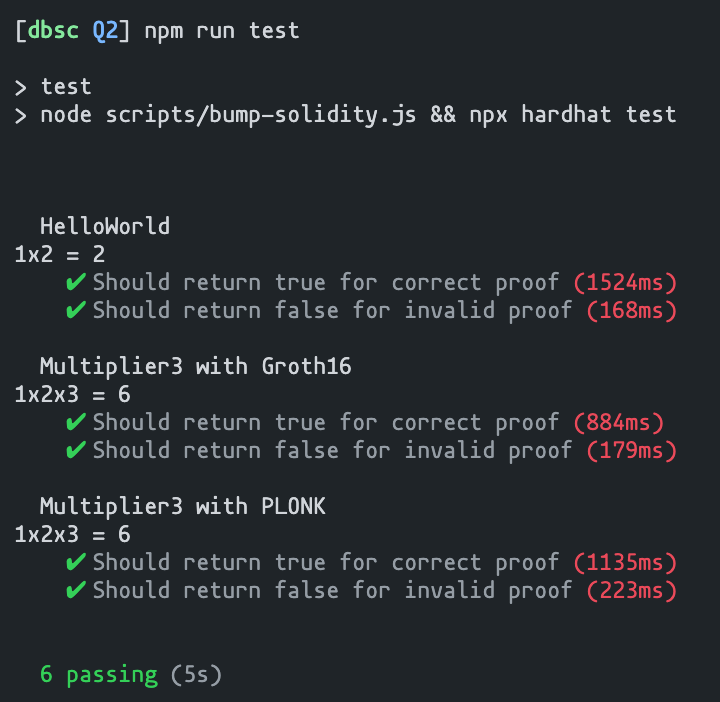
\includegraphics[width=0.7\textwidth]{tests.png}
    \caption*{Running tests for \texttt{Multiplier2} and \texttt{Multiplier3}.}
\end{figure}

\subsection*{Reading and designing circuits with circom}
\begin{itemize}
    \item \texttt{contracts/circuits/LessThan10.circom} implements a circuit that verifies an input is less than 10 using the \texttt{LessThan} template. Study how the template is used in this circuit. What does the 32 in Line 9 stand for? \par It means that the input to be compared can be at no bigger than 32 bit integers.
    \item What are the possible outputs for the LessThan template and what do they mean respectively? \par The outputs can be 0, if the result of the comparison was a false one, or 1, if it was indeed a true comparison.
    \item You can run \texttt{npm run test:fullProof} while inside the \texttt{zkPuzzles} directory to test your modified circuit. You are expected to encounter an error. Record the error, resolve it by modifying \texttt{project/zkPuzzles/scripts/compile-circuits.sh}, and explain why it has occurred and what you did to solve the error. \par
    \begin{figure}[h]
        \centering
        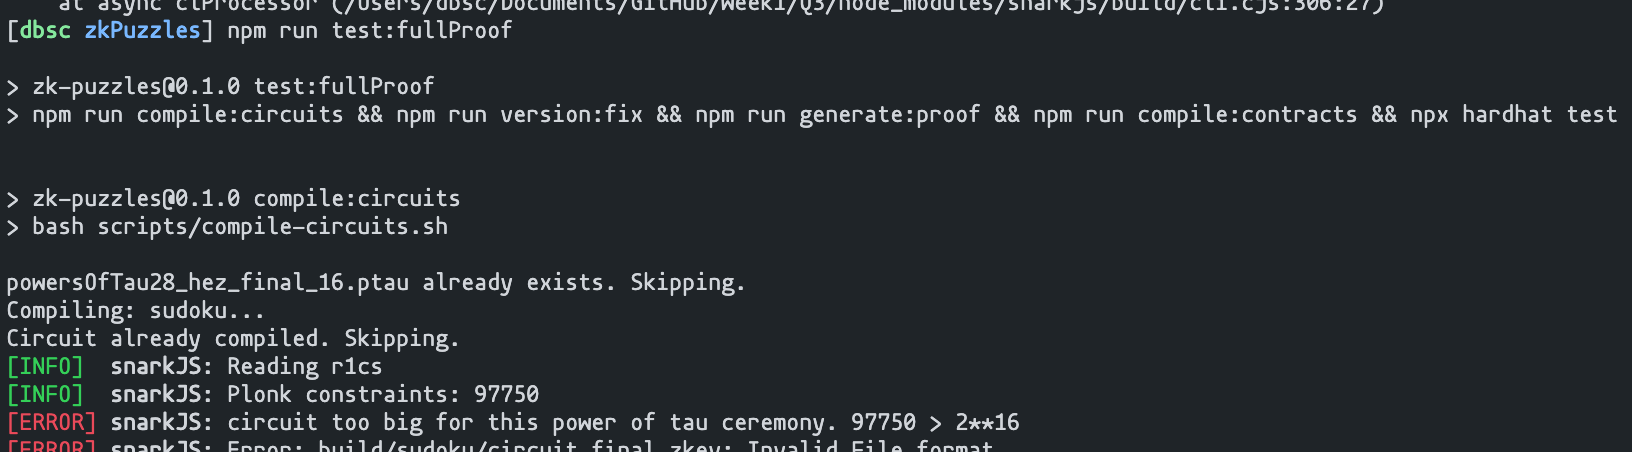
\includegraphics[width=0.8\textwidth]{error.png}
        \caption*{Sudoku circuit compilation error.}
    \end{figure}
    We can see that the error is very clear and tells us that the current ceremony can't accept a numbers of constraints bigger than $2^{16}$, so we need a bigger power of two, for example $2^{17} > 97750$. Thus we'll have to prepare our own cerimony with \texttt{snarkjs}. For this we'll use the following commands.
    \begin{lstlisting}[language=Bash]
# start a new powers of tau ceremony
snarkjs powersoftau new bn128 12 pot12_0000.ptau
# contribute to the ceremony
snarkjs powersoftau contribute pot12_0000.ptau pot12_0001.ptau
# prepare for phase 2
snarkjs powersoftau prepare phase2 pot12_0001.ptau pot12_final.ptau
    \end{lstlisting}
    We also modify \texttt{projects/zkPuzzles/scripts/compile-circuits.sh} so that it uses our newly generated powers of tau ceremony.
    \item Instead of using a brute force method to verify a sudoku puzzle solution, the circuit here uses the sum and sum of squares of each row, each column, and each “box” to prove the solution. What is/are the benefit(s) of this algorithmic implementation over the brute force implementation? \par It's faster, since it has a quadratic complexity on the size of the board, whereas the brute force has a cubic complexity over the board. This is possible since we know the range of the numbers, and the only way the sum of the numbers on a line, and the sum of the square of the numbers in a line may be equal to 45 and 315 respectively is if they are all distinct. We use the same idea for the inner boxes. In this way we can declare a sum variable instead of having another foor loop.
\end{itemize}

I have attempted the first bonus problem, and I was able to produce a code that uses the \texttt{circomlib-matrix} library but it throws an out of bounds error that I was not able to find a solution for in the current moment.
\end{document}
